%!TEX root = ../../super_main.tex

\section{Background Sensor Service}
\label{sec:background_sensor_service}
We have implemented a service, which we call \mono{BackgroundSensorService}, in order to facility non-intrusive data collection in the Android system.
This section includes some technical details about how services work in Android and how we have implemented our \mono{BackgroundSensorService}. 

\subsection{What is an Android service?}
A services in Android is an application component which encapsulates long running background processing or a way to provide access to a shared ressource. Services can be shared and can be configured run independently, i.e. running in a different process, from the graphical interface shown to users, which is ideal for our background data collection. Services have their own lifecycles and can be configured in many different ways. They can be configured as an API where the service itself has a short lifespan while serving some data or while performing a short task or they can be configured as a long running background task with its own complex behavior.
\\\\
% Message parsing
The Android framework supports two-way message parsing as a way of communication with a service when it runs in a different process. Message parsing makes it easy for the Android \mono{Activity} elements in the graphical and interactive part of the application to communicate with our \mono{BackgroundSensorService}.

% Boot receiver
% On Application start
\subsection{Service Start}
Our \mono{BackgroundSensorService} should ideally always be running, which does not imply that it is constantly using processing resources. We have implemented two measures to ensures that the service is running for as much time as possible. We have implemented an Android BroadcastReceiver, which upon receiving a system wide boot completed action (\mono{ACTION\_BOOT\_COMPLETED}), starts the service. The service is also attempted started every time the application is started, but is not started twice if the service is already running. 

\subsection{Snapshot Generation and Synchronization}
\label{sub:background_sensor_service_snapshot_generation_and_synchronization}

The background \mono{BackgroundSensorService} uses an independed timer for snapshot generation. The timer for snapshot generation is encapsulated in a class called \mono{SnapshotTimer} which is started whenever the service has an active running campaign which should generate snapshots. Timed tasks are then scheduled at a constant rate, generating snapshots, until the campaign is completed or stopped by the user.
\\\\
Before we send all available snapshots to the server we transform them to a JSON format, because JSON is humanly readable, decent for machine learning purposes, and because it has to have some well defined format when we send it, so it can be made sense of on the server. We use this because it is easy, instead of inventing our own format, but at the sacrifice of spending extra bandwidth of the participant to send it, which is rather bad. A better solution would be to use some format with few-to-no keys, where we have optimized how much space we use. 
\\\\
When we have converted the data to JSON, the actual synchronization of snapshots is done separately and is encapsulated in a class called \mono{SynchronizationManager}. This synchronization should ideally be done using as little network resources as possible, and thereby also save battery capacity. 
\\\\
An example of an Android API, or rather a library with Google APIs for Android, which could help optimize network usage, and the, would be the \mono{GCMNetworkManager}, which is an Android service, that can schedule encapsulated network tasks. \mono{GCMNetworkManager} \parencite{gcmnetworkmanager} handles batching of network tasks; retries; backoffs, in case a remote server is not responding or is busy; waiting for Wi-Fi, for bandwidth heavy communication; waiting with communication until the device is charging; and waiting until a radio becomes active, for instance by getting activated by another application. It does all of this based on parameters given to every encapsulated network tasks such as a desired time frame for the network communication and desired network or battery conditions.  
\\\\
Our \mono{SynchronizationManager} uses the \mono{GCMNetworkManager} to schedule a periodic task which attempts to synchronize gathered snapshots with the server at a fixed rate. Our periodic task is configured to override and removes the old pending tasks if it rescheduled but has not yet been executed. It is then up to the \mono{GCMNetworkManager} to determine when the task should be executed based parameters given with the task. Our task is configured to require that an unmetered connection, e.g. WiFi, is available before the task can be executed. 
\\\\
The \mono{GCMNetworkManager} incorporates radio based optimizations and will start all the pending tasks if the radio is active and a minimum time, as specified by the parameters, has elapsed. This minimizes unnecessary wake-ups of the radio and thus minimizes battery consumption. Using \mono{GCMNetworkManager} makes sense for network related operations which can be delayed in order to minimize battery consumption. Other network tasks which should happen instantly, such a refreshing the GUI with lists of campaigns from the server, are therefore not applicable to be optimized with \mono{GCMNetworkManager}. 

\subsection{Background Sensor Listening}
The \mono{BackgroundSensorService} is configured to have one thread, in a pool of threads, available per sensor type, i.e. per \mono{SensorProvider}, see \secref{sub:providing_sensor_data_implementation}, instance used in the service. This lets the scheduling of the gathering from the different \mono{SensorProvider} instances up to the underlying Java implementation of threads in a hope to run the different types of sensors and other data sources as independently as possible. Data is only collected from the \mono{SensorProvider} instances if the corresponding sensors are included in the currently active campaign and if the system is currently gathering a snapshot. There is no data collection activity in the \mono{BackgroundSensorService} unless a timed task for a snapshot is running. CPU resources, and thereby battery, are therefore only consumed on demand.
\\\\
We do not provide any real time guarantees but the different threads from the different streams of data should always be able to run unless they get starved by other processes in the system. Temporary starvation of the data collecting threads might result in missed updates from different data sources. 

\subsection{Concurrency Overview}
We have attempted to give an overview of the current processes and threads running in the mobile application in \figref{fig:system_currency_and_lifecycle} illustrated with a near UML Activity Diagram Syntax. We provide this overview so the communication between the different processes and communication in the application becomes more clear.
\\\\
As seen on the figure the system is split into two parts, namely an Android application part (GUI), and a Background Sensor Service part. The Android application is further split into two activities, namely the \emph{Main Activity} and the \emph{Questionnaire Activity}. As seen in \figref{fig:system_currency_and_lifecycle} the Main Activity lives until the participants closes it. During the life cycle of this activity the participant are able to subscribe to campaigns and cancel campaigns. Like the Main Activity the Questionnaire Activity lives until the questionnaire within is answered. However, the Questionnaire Activity might also expire if the delay from the expire timer ends before the participants have answered. 
\\\\
Both the Main Activity and the Questionnaire Activity is started by an Intent Handler as seen in the middle left in \figref{fig:system_currency_and_lifecycle}. The \emph{Start Main}-receiver, which starts the Main Activity, is signaled when the user opens it, for instance by clicking the application icon from the home screen of the device. The \emph{Start Questionnaire}-receiver is signaled by the Background Sensor Service.
\\\\
The Background Sensor Service, is the main controller of ensuring that the collection of snapshots is done accordingly to the campaign specified. This service is started, as seen in \figref{fig:system_currency_and_lifecycle} (the top right corner of the service), by the \emph{Application Start}-signal or the \emph{onBoot}-signal if it is not already running. These signals are sent when the application is installed or after the device boots respectively. When the service is running, it starts two asynchronous tasks, a task for gathering snapshots which is the most complicated part of this process, and a task for syncing the snapshots to the server, as described in \secref{sub:background_sensor_service_snapshot_generation_and_synchronization}. As seen in the lower left of the figure the synchronization task simply checks every \emph{Synchronization Delay} if there are any snapshots ready to be uploaded. The other task firstly checks if there are any active campaigns on the device. If this is the case, or if the user at any time joins a campaign this tasks starts gathering samples from the sensor specified for that campaign and signals the Questionnaire Activity to prompt for a label. When the sample gathering is done it it stored on the device. Whenever the questionnaire is answered by the participants this is attached to the corresponding snapshot. These stored snapshots are now ready to be uploaded by the synchronization task. When ever samples have been gathered the task goes back to the \emph{Active Campaign}-state and it gathers snapshots until it has gathered enough snapshots.

\begin{figure}[!htbp]
    \centering
    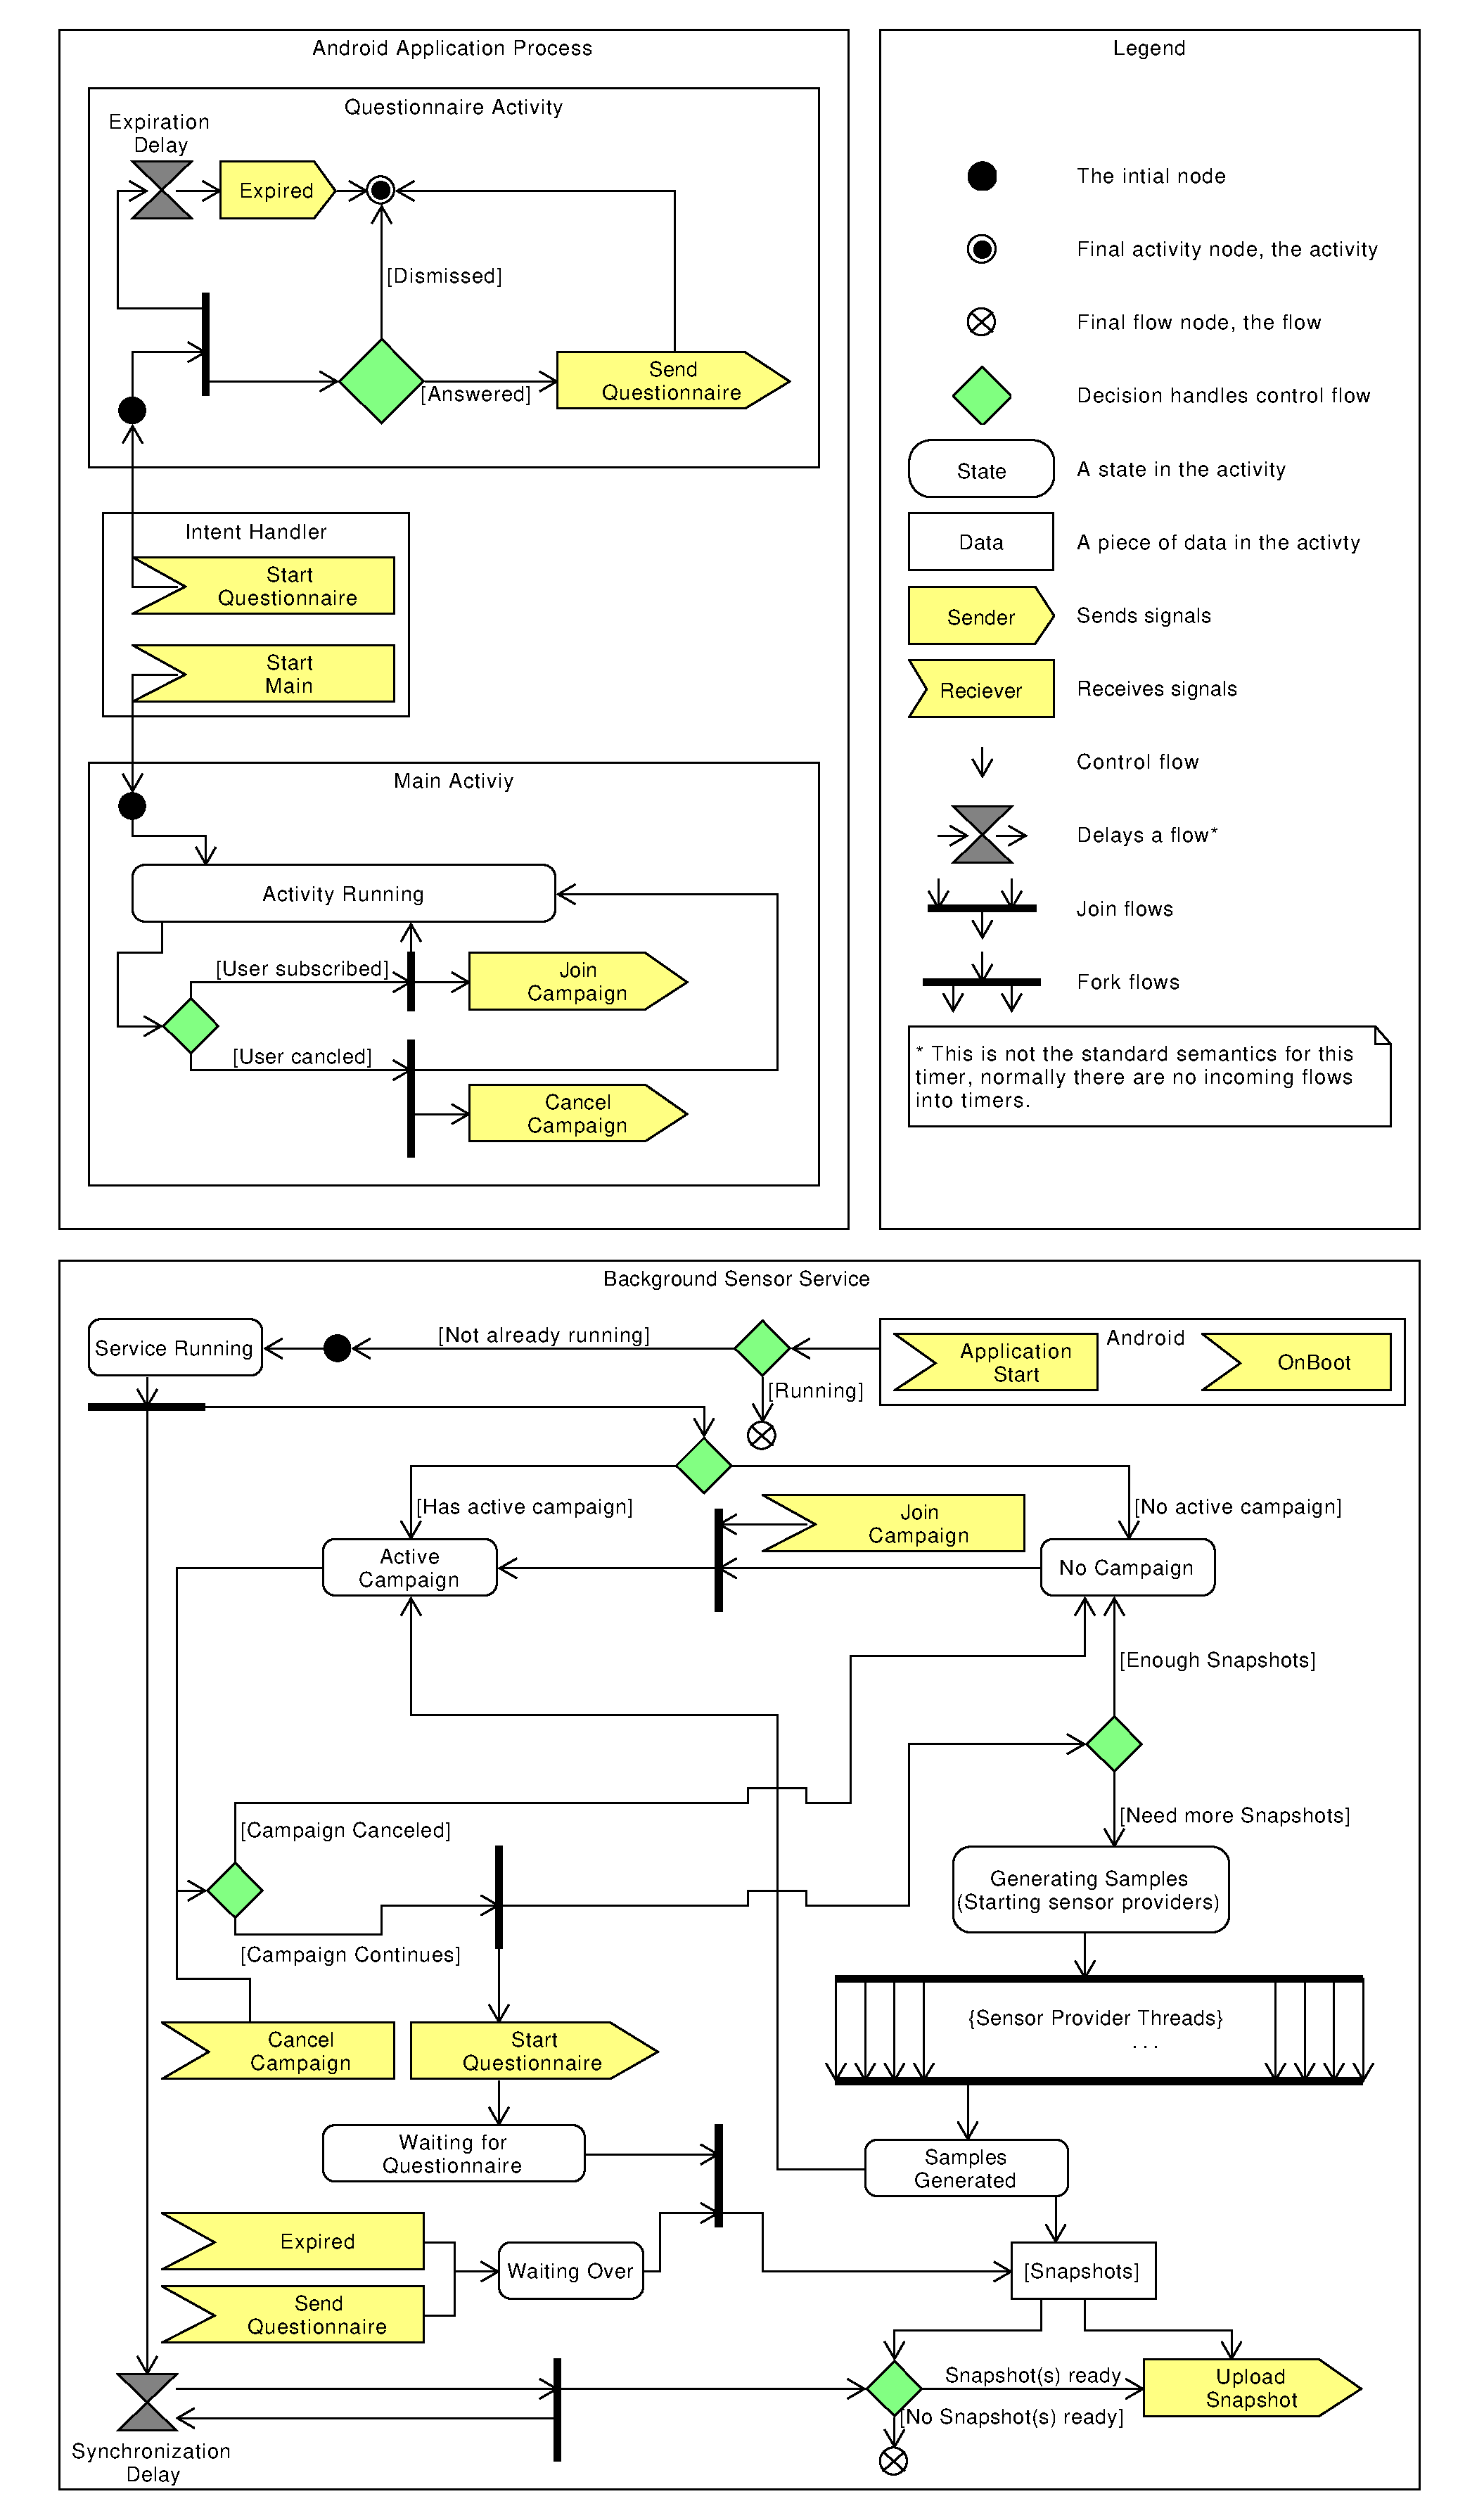
\includegraphics[width=\textwidth]{graphic/backgroundsensorservice/lifecyclestuff}
    \caption{An overview of the mobile Application Components.}
    \label{fig:system_currency_and_lifecycle}
\end{figure}
\FloatBarrier